\documentclass{article}
\usepackage{amsmath}
\usepackage{amsfonts}
\usepackage{booktabs}
\usepackage{graphicx}
\usepackage[section]{placeins}
\usepackage{longtable}

\newcommand{\albedo}{\alpha}
\newcommand{\transmission}{\tau}
\newcommand{\fref}[1]{Figure~\ref{#1}}
\newcommand{\eref}[1]{Equation~(\ref{#1})}
\newcommand{\tref}[1]{Table~\ref{#1}}
\newcommand{\sref}[1]{Section~\ref{#1}}

\begin{document}

\title{NE 770 Homework 2}
\author{William Dawn}
\maketitle

\section{Problem Statement}
  Two parameters that are often computed in the solution of the solution of 
  radiation transport problems are the total albedo ($\albedo$) defined to be 
  the fraction of incident particles which are reflected from a surface, and the 
  transmission factor ($\transmission$) defined to be the fraction of incident 
  particles which are transmitted through a medium. Write analog Monte Carlo 
  programs to compute the albedo and transmission factor for particles incident 
  on a slab with incident angular distribution given in \eref{eq:fofmu}.
  \begin{equation}
    \label{eq:fofmu}
    f(\mu) = (\beta + 2) \, \mu^{(\beta+1)} \qquad \beta > 0 \qquad \mu \in [0,1]
  \end{equation}

  You may assume scattering is isotropic in the lab system. Benchmark your
  solution against the following ``analytic'' results for this problem provided 
  in \tref{tab:analytic}. Examine the ``convergence'' of your solution as a 
  function of the number of particle histories.

  \begin{table}
    \caption{Reference Results.}
    \label{tab:analytic}
    \begin{center}
      \begin{tabular}{ccccc}
        \toprule
        $\lambda$ & $\beta$ & $c$ & $\albedo$ & $\transmission$ \\
        \midrule
        1 & 0 & 0.1 & 0.02075 & 0.2319  \\
        1 & 0 & 0.8 & 0.2802  & 0.4162  \\
        1 & 4 & 0.8 & 0.2350  & 0.4942  \\
        5 & 0 & 0.8 & 0.3417  & 0.02292 \\
        \bottomrule
      \end{tabular}
    \end{center}
  \end{table}

  Examine the performance of relative uncertainty in the mean
  ($\frac{\sigma_{\albedo}}{\albedo}$ \&
  $\frac{\sigma_{\transmission}}{\transmission}$) of your Monte Carlo simulation
  for scatter-to-total ratios of $c \in [0.1,0.99]$, slab thicknesses $\lambda
  \in [0,10]$ mean free paths, and $\beta \in [0,4]$.

\section{Solution}
  An analog Monte Carlo code was developed for the problem described. All
  reference results agree to within statistical uncertainty. It was determined
  that $10^6$ particles provided an acceptable answer. Therefore, all of the
  following problems are executed with one-million particles and relative
  uncertainty is measured. Alternatively, the problem could be run for a fixed
  relative uncertainty and the number of particles measured. As a demonstration
  of the simulation, the reference problem with $\lambda = 1$, $\beta = 0$, and
  $c = 0.8$ is analyzed in-depth as it has acceptable performance for both
  albedo and transmission factors.

  Results of this study are presented in \fref{fig:albedo_mean}, 
  \fref{fig:albedo_reluncertainty}, and \fref{fig:albedo_fom} for the albedo
  factor. Results for the transmission factor are presented in
  \fref{fig:transmission_mean}, \fref{fig:transmission_reluncertainty}, and
  \fref{fig:transmission_fom}. As expected, both albedo and transmission factors
  converge to the reference analytic transport calculation. Relative uncertainty
  in the mean decreases as $\frac{1}{\sqrt{N}}$ as expected and is quickly small
  enough for tolerance. The Figure of Merit (FOM) is calculated as \eref{eq:fom}
  and takes many particles before it reaches constant value.
  \begin{equation}
    \label{eq:fom}
    \text{FOM} = \frac{1}{\left(\frac{\sigma_z}{z}\right)^2 t}
  \end{equation}
  Where $t$ is the runtime. A larger FOM is preferable and the transmission FOM
  is larger for this problem. This implies that for this configuration, the
  transmission calculation is more efficient than the albedo calculation.

  Once the code is compared to reference results, a parametric study is
  conducted to analyze performance for various values of $\lambda$, $\beta$, and
  $c$. Each case was executed with one-million particles and relative
  uncertainties are compared. In total, 125 cases are analyzed. The data from
  these cases are included in \sref{sec:data} but is summarized briefly here.

  Maximum relative uncertainty in the albedo fraction was found for 
  $\lambda = 1$, $\beta = 4$, and $c = 0.1$. This implies high relative
  uncertainty for albedo problems in thin-slab geometry with forward-peaked flux
  and low scattering. Intuitively, these are problems with few particles
  reflected from the surface so there are few data points for calculating the
  albedo fraction. Minimum relative uncertainty in the albedo fraction was found
  for $\lambda = 10$, $\beta = 0$, and $c = 0.99$. This implies albedo fraction
  is easily calculated for thick-slab problems with isotropic particles and
  highly-scattering medium. This would create many reflected particles and many
  data points for calculating the albedo factor.

  Maximum relative uncertainty in the transmission fraction was found for
  $\lambda = 10$, $\beta = 0$, and $c = 0.1$. This problem is thick-slab with
  isotropic particles and highly-absorbing. There are few particles that
  ``escape'' the problem so there are few data points for calculating the
  transmission fraction. Minimum relative uncertainty in the transmission
  fraction was found for $\lambda = 1$, $\beta = 4$, and $c = 0.99$. This
  problem is thin-slab with highly forward-peaked particles and
  highly-scattering. This implies many particles exiting the slab at the far
  side and many data points for calculating the transmission fraction.

  \begin{figure}
    \centering
    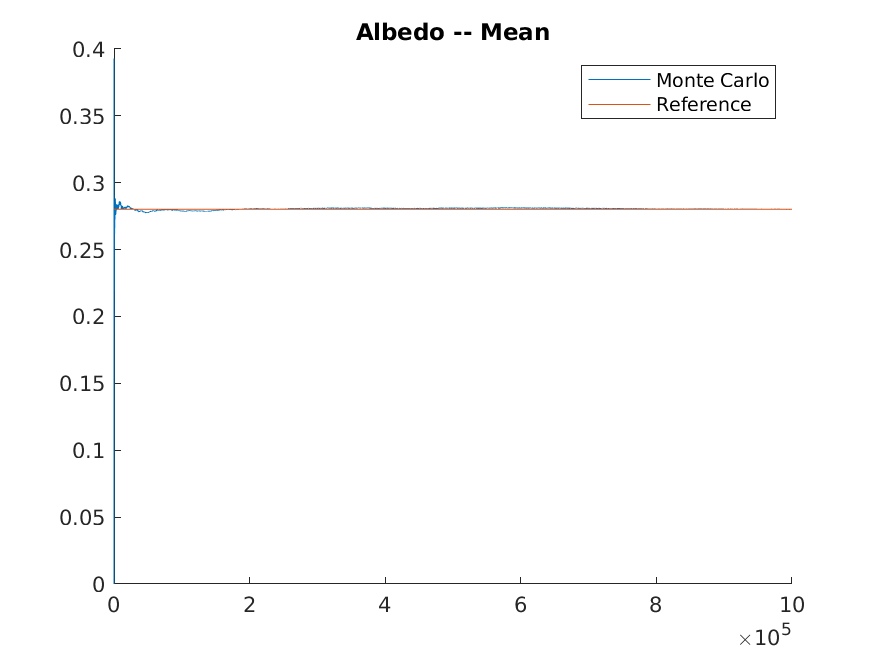
\includegraphics[width=0.8\textwidth]{albedo_mean}
    \caption{Albedo Fraction as a Function of Number of Samples.}
    \label{fig:albedo_mean}
  \end{figure}
  \begin{figure}
    \centering
    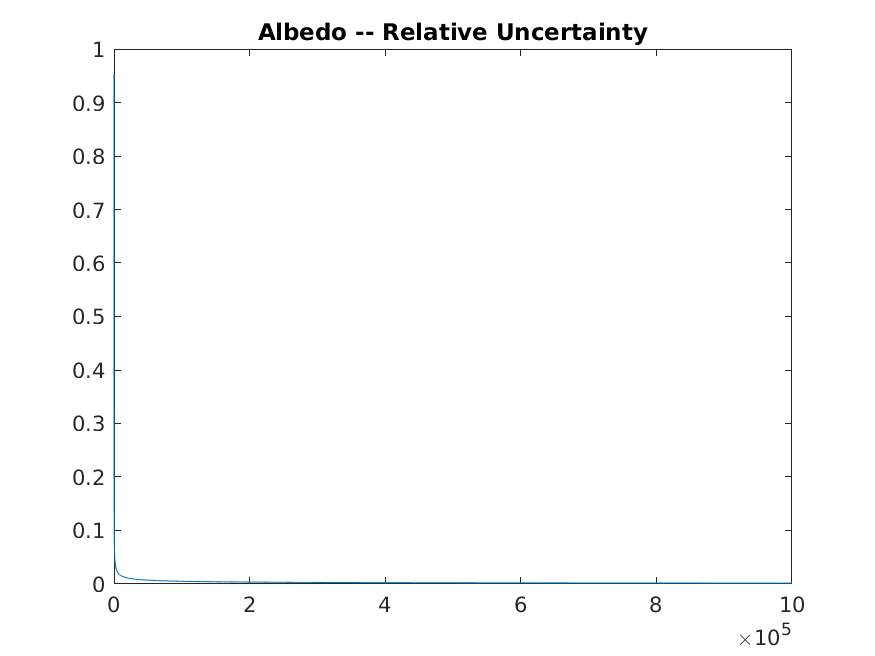
\includegraphics[width=0.8\textwidth]{albedo_reluncertainty}
    \caption{Relative Uncertainty in Albedo Fraction as a Function of Number 
      of Samples.}
    \label{fig:albedo_reluncertainty}
  \end{figure}
  \begin{figure}
    \centering
    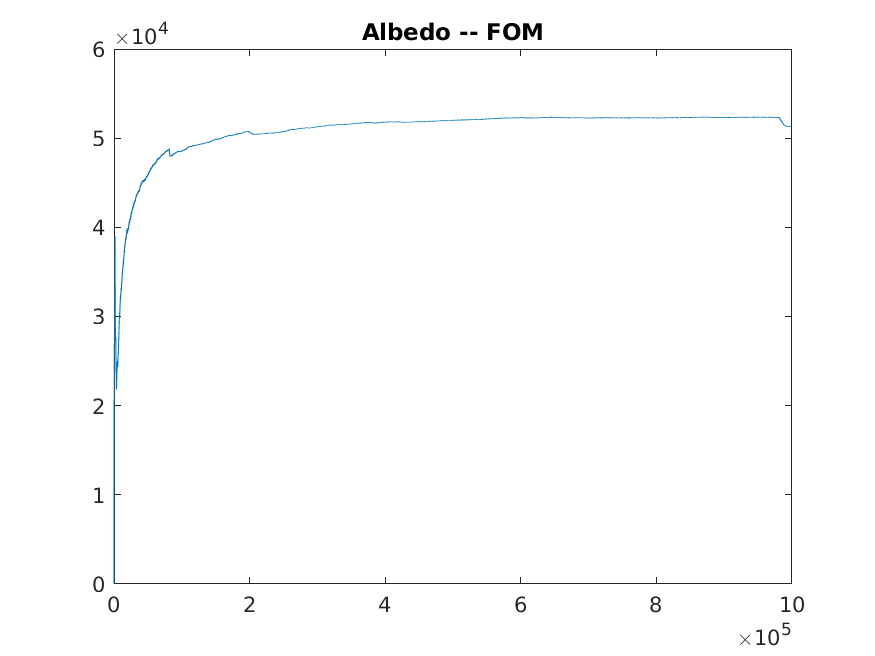
\includegraphics[width=0.8\textwidth]{albedo_fom}
    \caption{Albedo Fraction Figure of Merit as a Function of Number of 
      Samples.}
    \label{fig:albedo_fom}
  \end{figure}

  \begin{figure}
    \centering
    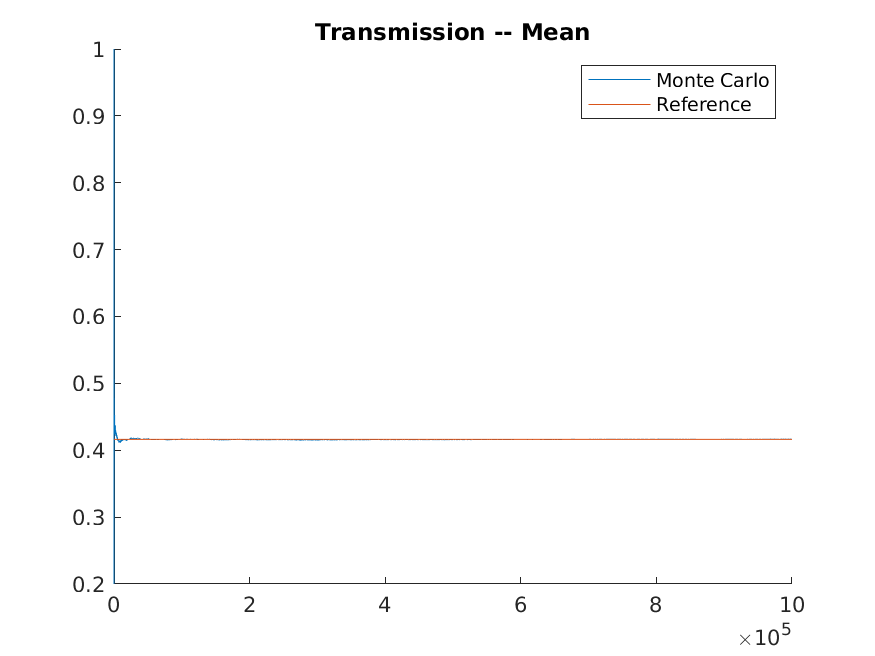
\includegraphics[width=0.8\textwidth]{transmission_mean}
    \caption{Transmission Fraction as a Function of Number of Samples.}
    \label{fig:transmission_mean}
  \end{figure}
  \begin{figure}
    \centering
    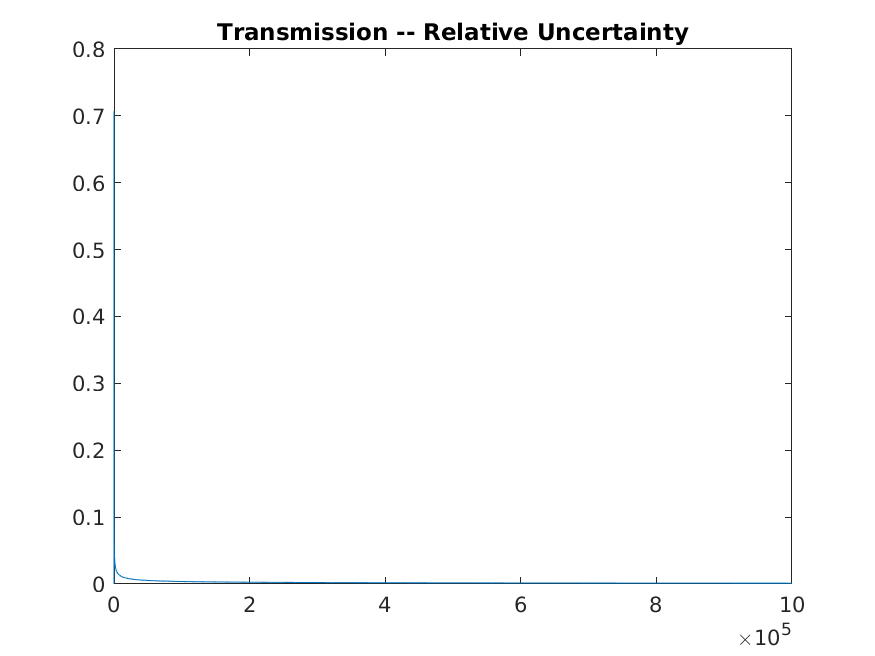
\includegraphics[width=0.8\textwidth]{transmission_reluncertainty}
    \caption{Relative Uncertainty in Transmission Fraction as a Function of Number 
      of Samples.}
    \label{fig:transmission_reluncertainty}
  \end{figure}
  \begin{figure}
    \centering
    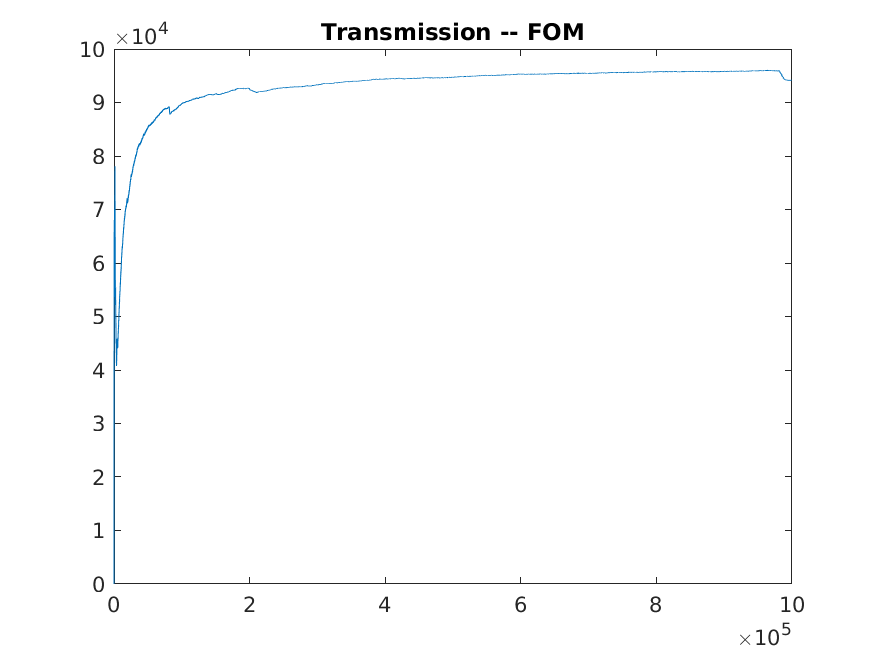
\includegraphics[width=0.8\textwidth]{transmission_fom}
    \caption{Transmission Fraction Figure of Merit as a Function of Number of 
      Samples.}
    \label{fig:transmission_fom}
  \end{figure}


\section{Data}
  \label{sec:data}
  \begin{longtable}{ccccccc}
    \toprule
    $\lambda$ & $\beta$ & $c$ & $\albedo$ &
    $\frac{\sigma_{\albedo}}{\albedo}$ &
    $\transmission$ & $\frac{\sigma_{\transmission}}{\transmission}$ \\
    \midrule
    1.000& 0.000& 0.100&0.020806&0.006860&0.232535&0.001817\\
    1.000& 0.000& 0.323&0.076220&0.003481&0.266141&0.001661\\
    1.000& 0.000& 0.545&0.151308&0.002368&0.318973&0.001461\\
    1.000& 0.000& 0.767&0.260064&0.001687&0.400348&0.001224\\
    1.000& 0.000& 0.990&0.436282&0.001137&0.544119&0.000915\\
    1.000& 1.000& 0.100&0.019045&0.007177&0.270834&0.001641\\
    1.000& 1.000& 0.323&0.069604&0.003656&0.306063&0.001506\\
    1.000& 1.000& 0.545&0.138741&0.002492&0.355927&0.001345\\
    1.000& 1.000& 0.767&0.239090&0.001784&0.437126&0.001135\\
    1.000& 1.000& 0.990&0.405187&0.001212&0.576086&0.000858\\
    1.000& 2.000& 0.100&0.017905&0.007406&0.293937&0.001550\\
    1.000& 2.000& 0.323&0.065938&0.003764&0.330461&0.001423\\
    1.000& 2.000& 0.545&0.132592&0.002558&0.378090&0.001283\\
    1.000& 2.000& 0.767&0.228768&0.001836&0.457535&0.001089\\
    1.000& 2.000& 0.990&0.388136&0.001256&0.593823&0.000827\\
    1.000& 3.000& 0.100&0.017050&0.007593&0.310279&0.001491\\
    1.000& 3.000& 0.323&0.063679&0.003835&0.344243&0.001380\\
    1.000& 3.000& 0.545&0.128002&0.002610&0.393023&0.001243\\
    1.000& 3.000& 0.767&0.221903&0.001873&0.470794&0.001060\\
    1.000& 3.000& 0.990&0.377342&0.001285&0.604901&0.000808\\
    1.000& 4.000& 0.100&0.016988&0.007607&0.319994&0.001458\\
    1.000& 4.000& 0.323&0.062645&0.003868&0.354481&0.001349\\
    1.000& 4.000& 0.545&0.125545&0.002639&0.403674&0.001215\\
    1.000& 4.000& 0.767&0.217819&0.001895&0.479288&0.001042\\
    1.000& 4.000& 0.990&0.369545&0.001306&0.612906&0.000795\\
    3.250& 0.000& 0.100&0.021591&0.006732&0.015145&0.008064\\
    3.250& 0.000& 0.323&0.081089&0.003366&0.020973&0.006832\\
    3.250& 0.000& 0.545&0.166045&0.002241&0.033825&0.005345\\
    3.250& 0.000& 0.767&0.308888&0.001496&0.069561&0.003657\\
    3.250& 0.000& 0.990&0.678814&0.000688&0.260270&0.001686\\
    3.250& 1.000& 0.100&0.020231&0.006959&0.019107&0.007165\\
    3.250& 1.000& 0.323&0.075305&0.003504&0.025916&0.006131\\
    3.250& 1.000& 0.545&0.155426&0.002331&0.039438&0.004935\\
    3.250& 1.000& 0.767&0.292604&0.001555&0.078020&0.003438\\
    3.250& 1.000& 0.990&0.659597&0.000718&0.278079&0.001611\\
    3.250& 2.000& 0.100&0.018897&0.007205&0.021942&0.006676\\
    3.250& 2.000& 0.323&0.071977&0.003591&0.029371&0.005749\\
    3.250& 2.000& 0.545&0.150024&0.002380&0.043956&0.004664\\
    3.250& 2.000& 0.767&0.283730&0.001589&0.083804&0.003306\\
    3.250& 2.000& 0.990&0.648622&0.000736&0.288440&0.001571\\
    3.250& 3.000& 0.100&0.018210&0.007343&0.024901&0.006258\\
    3.250& 3.000& 0.323&0.070194&0.003640&0.031770&0.005521\\
    3.250& 3.000& 0.545&0.145876&0.002420&0.046925&0.004507\\
    3.250& 3.000& 0.767&0.277981&0.001612&0.087558&0.003228\\
    3.250& 3.000& 0.990&0.640866&0.000749&0.295749&0.001543\\
    3.250& 4.000& 0.100&0.017910&0.007405&0.026147&0.006103\\
    3.250& 4.000& 0.323&0.068603&0.003685&0.033920&0.005337\\
    3.250& 4.000& 0.545&0.143488&0.002443&0.049693&0.004373\\
    3.250& 4.000& 0.767&0.274172&0.001627&0.091357&0.003154\\
    3.250& 4.000& 0.990&0.635727&0.000757&0.300876&0.001524\\
    5.500& 0.000& 0.100&0.021835&0.006693&0.001156&0.029395\\
    5.500& 0.000& 0.323&0.081660&0.003353&0.001864&0.023140\\
    5.500& 0.000& 0.545&0.167151&0.002232&0.003833&0.016121\\
    5.500& 0.000& 0.767&0.310357&0.001491&0.012527&0.008878\\
    5.500& 0.000& 0.990&0.747520&0.000581&0.155373&0.002332\\
    5.500& 1.000& 0.100&0.020014&0.006998&0.001589&0.025066\\
    5.500& 1.000& 0.323&0.074855&0.003516&0.002392&0.020422\\
    5.500& 1.000& 0.545&0.155698&0.002329&0.004625&0.014670\\
    5.500& 1.000& 0.767&0.293818&0.001550&0.014137&0.008351\\
    5.500& 1.000& 0.990&0.733109&0.000603&0.166348&0.002239\\
    5.500& 2.000& 0.100&0.019069&0.007172&0.001907&0.022878\\
    5.500& 2.000& 0.323&0.072479&0.003577&0.002804&0.018858\\
    5.500& 2.000& 0.545&0.150463&0.002376&0.005074&0.014003\\
    5.500& 2.000& 0.767&0.285391&0.001582&0.015464&0.007979\\
    5.500& 2.000& 0.990&0.724813&0.000616&0.172359&0.002191\\
    5.500& 3.000& 0.100&0.018315&0.007321&0.002057&0.022026\\
    5.500& 3.000& 0.323&0.070372&0.003635&0.003089&0.017965\\
    5.500& 3.000& 0.545&0.146284&0.002416&0.005428&0.013536\\
    5.500& 3.000& 0.767&0.279608&0.001605&0.016517&0.007716\\
    5.500& 3.000& 0.990&0.720214&0.000623&0.176422&0.002161\\
    5.500& 4.000& 0.100&0.018033&0.007379&0.002297&0.020841\\
    5.500& 4.000& 0.323&0.068944&0.003675&0.003263&0.017478\\
    5.500& 4.000& 0.545&0.143935&0.002439&0.005966&0.012908\\
    5.500& 4.000& 0.767&0.276835&0.001616&0.016719&0.007669\\
    5.500& 4.000& 0.990&0.714438&0.000632&0.180719&0.002129\\
    7.750& 0.000& 0.100&0.021684&0.006717&0.000093&0.103690\\
    7.750& 0.000& 0.323&0.081226&0.003363&0.000171&0.076465\\
    7.750& 0.000& 0.545&0.167059&0.002233&0.000435&0.047936\\
    7.750& 0.000& 0.767&0.310515&0.001490&0.002283&0.020905\\
    7.750& 0.000& 0.990&0.774307&0.000540&0.100075&0.002999\\
    7.750& 1.000& 0.100&0.019692&0.007056&0.000128&0.088383\\
    7.750& 1.000& 0.323&0.075338&0.003503&0.000219&0.067566\\
    7.750& 1.000& 0.545&0.155696&0.002329&0.000534&0.043263\\
    7.750& 1.000& 0.767&0.294505&0.001548&0.002551&0.019774\\
    7.750& 1.000& 0.990&0.761828&0.000559&0.107120&0.002887\\
    7.750& 2.000& 0.100&0.018870&0.007211&0.000168&0.077145\\
    7.750& 2.000& 0.323&0.072245&0.003584&0.000272&0.060626\\
    7.750& 2.000& 0.545&0.150546&0.002375&0.000638&0.039578\\
    7.750& 2.000& 0.767&0.285326&0.001583&0.002753&0.019033\\
    7.750& 2.000& 0.990&0.754113&0.000571&0.111022&0.002830\\
    7.750& 3.000& 0.100&0.018738&0.007237&0.000188&0.072926\\
    7.750& 3.000& 0.323&0.070043&0.003644&0.000323&0.055633\\
    7.750& 3.000& 0.545&0.147105&0.002408&0.000613&0.040377\\
    7.750& 3.000& 0.767&0.279614&0.001605&0.003027&0.018148\\
    7.750& 3.000& 0.990&0.748959&0.000579&0.113638&0.002793\\
    7.750& 4.000& 0.100&0.018276&0.007329&0.000240&0.064542\\
    7.750& 4.000& 0.323&0.069440&0.003661&0.000331&0.054956\\
    7.750& 4.000& 0.545&0.144128&0.002437&0.000721&0.037229\\
    7.750& 4.000& 0.767&0.276275&0.001619&0.003041&0.018106\\
    7.750& 4.000& 0.990&0.746133&0.000583&0.115442&0.002768\\
   10.000& 0.000& 0.100&0.021701&0.006714&0.000011&0.301510\\
   10.000& 0.000& 0.323&0.081451&0.003358&0.000013&0.277348\\
   10.000& 0.000& 0.545&0.166594&0.002237&0.000041&0.156171\\
   10.000& 0.000& 0.767&0.310796&0.001489&0.000415&0.049078\\
   10.000& 0.000& 0.990&0.784856&0.000524&0.066600&0.003744\\
   10.000& 1.000& 0.100&0.019767&0.007042&0.000015&0.258197\\
   10.000& 1.000& 0.323&0.075872&0.003490&0.000026&0.196114\\
   10.000& 1.000& 0.545&0.156465&0.002322&0.000059&0.130185\\
   10.000& 1.000& 0.767&0.293899&0.001550&0.000458&0.046716\\
   10.000& 1.000& 0.990&0.773283&0.000541&0.071359&0.003607\\
   10.000& 2.000& 0.100&0.019281&0.007132&0.000015&0.258197\\
   10.000& 2.000& 0.323&0.071752&0.003597&0.000020&0.223605\\
   10.000& 2.000& 0.545&0.150076&0.002380&0.000064&0.124996\\
   10.000& 2.000& 0.767&0.284465&0.001586&0.000520&0.043841\\
   10.000& 2.000& 0.990&0.766062&0.000553&0.074085&0.003535\\
   10.000& 3.000& 0.100&0.018470&0.007290&0.000020&0.223605\\
   10.000& 3.000& 0.323&0.069755&0.003652&0.000026&0.196114\\
   10.000& 3.000& 0.545&0.146448&0.002414&0.000074&0.116243\\
   10.000& 3.000& 0.767&0.279658&0.001605&0.000534&0.043263\\
   10.000& 3.000& 0.990&0.762311&0.000558&0.075509&0.003499\\
   10.000& 4.000& 0.100&0.017998&0.007387&0.000014&0.267259\\
   10.000& 4.000& 0.323&0.068550&0.003686&0.000023&0.208512\\
   10.000& 4.000& 0.545&0.143776&0.002440&0.000080&0.111799\\
   10.000& 4.000& 0.767&0.275980&0.001620&0.000575&0.041691\\
   10.000& 4.000& 0.990&0.759606&0.000563&0.076623&0.003471\\
   \bottomrule
  \end{longtable}

\end{document}
